\documentclass[11pt,a4paper]{article}
\usepackage[T1]{fontenc}
\usepackage[utf8]{inputenc}
\usepackage{lmodern,microtype}
\usepackage[margin=23mm]{geometry}
\usepackage{amsmath,amssymb,booktabs,array,graphicx,siunitx,xurl,xspace}
\usepackage[numbers,sort&compress]{natbib}
\usepackage[colorlinks=true,linkcolor=blue!50!black,citecolor=blue!50!black,urlcolor=blue!50!black]{hyperref}
\usepackage{xcolor,placeins,tikz}
\usetikzlibrary{decorations.pathmorphing,arrows.meta,positioning}
\graphicspath{{figures/}}
% Selected definitions imported from the ITACA manuscript on 2026-10-22.
% Source: /Users/jjgomezcadenas/Papers/itaca/pool/NextDefs.tex
% Used by itacaRevisited.tex alongside pool/NextLatexPackagesBase.tex.
% Local copy: compiling this note does not require the external directory.
% Preserve source macro names and notation; omit numerical design inputs,
% run-specific measurements, draft labels and conflicting SI unit aliases.
\usepackage{siunitx,xspace}
\sisetup{separate-uncertainty=true}

% Double-beta decay
\newcommand{\bb}{\ensuremath{\beta\beta}}
\newcommand{\bbonu}{\ensuremath{\beta\beta0\nu}}
\newcommand{\bbtnu}{\ensuremath{\beta\beta2\nu}}
\newcommand{\Qbb}{\ensuremath{Q_{\beta\beta}}}
\newcommand{\mbb}{\ensuremath{m_{\beta\beta}}}
\newcommand{\Tonu}{\ensuremath{T_{1/2}^{0\nu}}}
\newcommand{\Ttnu}{\ensuremath{T_{1/2}^{2\nu}}}
\newcommand{\Monu}{\ensuremath{\Big|M_{0\nu}\Big|}}
\newcommand{\Mtnu}{\ensuremath{\Big|M_{2\nu}\Big|}}
\newcommand{\Gonu}{\ensuremath{G_{0\nu}(\Qbb, Z)}}
\newcommand{\Gtnu}{\ensuremath{G_{2\nu}(\Qbb, Z)}}

% Isotopes and ion species
\newcommand{\XE}{\ensuremath{{}^{136}\rm Xe}}
\newcommand{\XEO}{\ensuremath{^{137}}Xe}
\newcommand{\BI}{\ensuremath{{}^{214}\rm Bi}}
\newcommand{\TL}{\ensuremath{{}^{208}\rm{Tl}}}
\newcommand{\KR}{\ensuremath{^{83m}\mathrm{Kr}}\xspace}
\newcommand{\Xe}[1]{\ensuremath{^{#1}\mathrm{Xe}}\xspace}
\newcommand{\Bi}[1]{\ensuremath{^{#1}\mathrm{Bi}}\xspace}
\newcommand{\Tl}[1]{\ensuremath{^{#1}\mathrm{Tl}}\xspace}
\newcommand{\Kr}[1]{\ensuremath{^{#1}\mathrm{Kr}}\xspace}
\newcommand{\xetp}{\ensuremath{{\rm Xe_2^{+}}}}
\newcommand{\batp}{\ensuremath{{\rm Ba^{2+}}}}
\newcommand{\nhfp}{\ensuremath{{\rm NH_4^{+}}}}
\newcommand{\nht}{\ensuremath{{\rm NH_3}}}

% Detector names and terminology
\newcommand{\NEW}{NEXT-White}
\newcommand{\NEXT}{NEXT-100}
\newcommand{\GXeEL}{GXeEL}
\newcommand{\HPXe}{HPXe}
\newcommand{\HPXeEL}{HPXe-EL}
\newcommand{\TM}{\emph{Topmetal}\xspace}

% Signals, transport and statistical notation
\newcommand{\tz}{\ensuremath{t_0}}
\newcommand{\sone}{\ensuremath{S_1}}
\newcommand{\stwo}{\ensuremath{S_2}}
\newcommand{\nph}{\ensuremath{n_\gamma}}
\newcommand{\VDR}{\ensuremath{v_d}}
\newcommand{\VD}{\ensuremath{v_d}}
\newcommand{\REF}{\ensuremath{\frac{E}{P}}}
\newcommand{\REY}{\ensuremath{\frac{Y}{P}}}
\newcommand{\chitwo}{\ensuremath{\chi^2}}
\newcommand{\SigmaE}{\ensuremath{\sigma_E / E}}
\newcommand{\stat}{\textrm{(stat.)}}
\newcommand{\sys}{\textrm{(sys.)}}

% Reference and table helpers
\newcommand{\fig}{figure}
\newcommand{\eq}{equation}
\newcommand{\tab}{table}
\newcommand{\Fig}{Figure}
\newcommand{\Eq}{Equation}
\newcommand{\Tab}{Table}
\newcommand{\minitab}[2][l]{\begin{tabular}{#1}#2\end{tabular}}

% Generated by notes/physics/figures/build_bi214_floor.py from
%   results/iitaca/II_L1000_D500_bi214_floor/floor.h5  sha256 80693f6c46acc17689b9d8588869e9dca7bc159b14b9bd86635f03e3386a6c12
%   results/iitaca/II_L1000_D500_pitch_comparison/comparison.h5  sha256 e5178e22d9fa58fcc5926b38e60b836e19af593c777ce8bae2bad03529722642
%   results/iitaca/II_L1000_D500_P2_bi214_truth/summary.h5  sha256 54df7c7cdd38a57d560a151587e6f3cb54d0bfb6a986cbd5562da1389a6b5764
\newcommand{\BiGenerated}{40{,}000{,}000}
\newcommand{\BiSaved}{1{,}271{,}276}
\newcommand{\BiTrigger}{162{,}982}
\newcommand{\BiROI}{31{,}641}
\newcommand{\BiSelected}{7{,}640}
\newcommand{\BiTrackFraction}{24.1}
\newcommand{\VetoGamma}{1{,}022{,}579}
\newcommand{\VetoGammaFrac}{80}
\newcommand{\VetoEL}{68{,}808}
\newcommand{\VetoFrame}{16{,}905}
\newcommand{\TriggerFrac}{12.8}
\newcommand{\RoiFrac}{19.4}
\newcommand{\EtwoThreshold}{177.7}
\newcommand{\BiEtwo}{11.8}
\newcommand{\BiEtwoErr}{0.4}
\newcommand{\SeEtwo}{6.0}
\newcommand{\SeEtwoErr}{0.1}
\newcommand{\SeEtwoEvents}{92{,}908}
\newcommand{\BiNet}{3.98}
\newcommand{\BiNetErr}{0.22}
\newcommand{\BiNetPassed}{304}
\newcommand{\SeNet}{1.34}
\newcommand{\SeNetErr}{0.10}
\newcommand{\SeNetPassed}{168}
\newcommand{\SeNetEvents}{12{,}523}
\newcommand{\BiNetRatio}{3.0}
\newcommand{\PhotEvents}{6{,}943}
\newcommand{\PhotPassed}{120}
\newcommand{\PhotNet}{1.73}
\newcommand{\PhotNetErr}{0.16}
\newcommand{\ComptEvents}{697}
\newcommand{\ComptPassed}{184}
\newcommand{\ComptNet}{26.4}
\newcommand{\ComptNetErr}{1.7}
\newcommand{\ComptShareSelected}{9.1}
\newcommand{\ComptSharePassed}{61}
\newcommand{\DistAEvents}{268}
\newcommand{\DistAPassed}{111}
\newcommand{\DistANet}{41.4}
\newcommand{\DistANetErr}{3.0}
\newcommand{\DistAEtwo}{76}
\newcommand{\DistBEvents}{305}
\newcommand{\DistBPassed}{64}
\newcommand{\DistBNet}{21.0}
\newcommand{\DistBNetErr}{2.3}
\newcommand{\DistBEtwo}{73}
\newcommand{\DistCEvents}{124}
\newcommand{\DistCPassed}{9}
\newcommand{\DistCNet}{7.3}
\newcommand{\DistCNetErr}{2.3}
\newcommand{\DistCEtwo}{67}
\newcommand{\DistAShareSelected}{3.5}
\newcommand{\DistAContribution}{1.45}
\newcommand{\DistBContribution}{0.84}
\newcommand{\DistASharePassed}{37}
\newcommand{\DistARejection}{1.9}
\newcommand{\XrayNoneNet}{1.31}
\newcommand{\XrayNoneEvents}{2{,}510}
\newcommand{\XrayNearNet}{2.18}
\newcommand{\XrayNearEvents}{2{,}800}
\newcommand{\ExpectedNet}{4.47}
\newcommand{\ExpectedNetErr}{0.28}
\newcommand{\ExcessEvents}{202}
\newcommand{\ComptExcess}{175}
\newcommand{\ComptLeadCompton}{173}
\newcommand{\ComptCentreMedianPassed}{7}
\newcommand{\ComptCentreMedianAll}{7}
\newcommand{\ComptCentreNinetyPassed}{14}
\newcommand{\ComptLtFour}{38}
\newcommand{\ThirdPureOne}{1.04}
\newcommand{\ThirdPureOneErr}{0.16}
\newcommand{\ThirdPureOneSigma}{0.42}
\newcommand{\ThirdPureOneEvents}{4{,}136}
\newcommand{\ThirdPureOneLo}{0}
\newcommand{\ThirdPureOneHi}{33}
\newcommand{\ThirdPureOneSig}{79.2}
\newcommand{\ThirdPureTwo}{1.46}
\newcommand{\ThirdPureTwoErr}{0.18}
\newcommand{\ThirdPureTwoSigma}{0.69}
\newcommand{\ThirdPureTwoEvents}{4{,}234}
\newcommand{\ThirdPureTwoLo}{33}
\newcommand{\ThirdPureTwoHi}{63}
\newcommand{\ThirdPureTwoSig}{80.2}
\newcommand{\ThirdPureThree}{1.52}
\newcommand{\ThirdPureThreeErr}{0.19}
\newcommand{\ThirdPureThreeSigma}{0.88}
\newcommand{\ThirdPureThreeEvents}{4{,}153}
\newcommand{\ThirdPureThreeLo}{63}
\newcommand{\ThirdPureThreeHi}{95}
\newcommand{\ThirdPureThreeSig}{80.6}
\newcommand{\ThirdPureAll}{1.34}
\newcommand{\ThirdPureAllErr}{0.10}
\newcommand{\ThirdPureFullSigma}{1.00}
\newcommand{\ThirdHybridOne}{0.99}
\newcommand{\ThirdHybridOneErr}{0.20}
\newcommand{\ThirdHybridOneSigma}{0.59}
\newcommand{\ThirdHybridOneEvents}{2{,}520}
\newcommand{\ThirdHybridOneLo}{0}
\newcommand{\ThirdHybridOneHi}{44}
\newcommand{\ThirdHybridOneSig}{79.6}
\newcommand{\ThirdHybridTwo}{1.46}
\newcommand{\ThirdHybridTwoErr}{0.24}
\newcommand{\ThirdHybridTwoSigma}{0.96}
\newcommand{\ThirdHybridTwoEvents}{2{,}463}
\newcommand{\ThirdHybridTwoLo}{44}
\newcommand{\ThirdHybridTwoHi}{84}
\newcommand{\ThirdHybridTwoSig}{80.2}
\newcommand{\ThirdHybridThree}{1.14}
\newcommand{\ThirdHybridThreeErr}{0.21}
\newcommand{\ThirdHybridThreeSigma}{1.22}
\newcommand{\ThirdHybridThreeEvents}{2{,}458}
\newcommand{\ThirdHybridThreeLo}{84}
\newcommand{\ThirdHybridThreeHi}{125}
\newcommand{\ThirdHybridThreeSig}{80.2}
\newcommand{\ThirdHybridAll}{1.20}
\newcommand{\ThirdHybridAllErr}{0.13}
\newcommand{\ThirdHybridFullSigma}{1.36}
\newcommand{\GasDensity}{99.2}
\newcommand{\BackscatterKeV}{231}
\newcommand{\NinetyKeV}{423}
\newcommand{\BackscatterLambda}{35}
\newcommand{\LambdaThree}{56}
\newcommand{\PtenThree}{1.8}
\newcommand{\LambdaFour}{82}
\newcommand{\PtenFour}{1.2}
\newcommand{\LambdaFive}{104}
\newcommand{\PtenFive}{1.0}
\newcommand{\LineLambda}{260}
\newcommand{\VoxEvents}{31{,}641}
\newcommand{\VoxSelected}{6{,}764}
\newcommand{\VoxFraction}{21.4}
\newcommand{\VoxBoth}{6{,}620}
\newcommand{\VoxOnly}{144}
\newcommand{\ReadoutOnly}{1{,}020}
\newcommand{\VoxReadoutSelected}{7{,}640}
\newcommand{\VoxBoxDiff}{0.001}
\newcommand{\VoxComptKept}{459}
\newcommand{\VoxComptKeptFrac}{66}
\newcommand{\VoxComptPassKept}{150}
\newcommand{\VoxComptPass}{184}
\newcommand{\VoxDistAKept}{86}
\newcommand{\VoxDistAEvents}{268}
\newcommand{\VoxDistBKept}{65}
\newcommand{\VoxDistBEvents}{305}
\newcommand{\VoxDistCKept}{23}
\newcommand{\VoxDistCEvents}{124}
\newcommand{\VoxPhotKept}{89}
\newcommand{\VoxPassKept}{258}
\newcommand{\VoxNonComptPassKept}{108}
\newcommand{\VoxRejDeposit}{1{,}007}
\newcommand{\ReadoutRejDeposit}{131}
\newcommand{\DispASecondKeV}{305}
\newcommand{\DispAPhotonPath}{1}
\newcommand{\DispBSecondKeV}{400}
\newcommand{\DispBPhotonPath}{5}
\newcommand{\DispRSecondKeV}{236}
\newcommand{\DispRPhotonPath}{31}
\newcommand{\BiThirdOneLo}{0}
\newcommand{\BiThirdOneHi}{30}
\newcommand{\BiThirdOneSel}{23.4}
\newcommand{\BiThirdOneVox}{21.9}
\newcommand{\BiThirdOneNet}{3.94}
\newcommand{\BiThirdOneNetErr}{0.39}
\newcommand{\BiThirdOneCompt}{203}
\newcommand{\BiThirdOneComptShare}{8.2}
\newcommand{\BiThirdOneComptNet}{29}
\newcommand{\BiThirdOneComptNetErr}{3}
\newcommand{\BiThirdOnePerRoi}{9.20}
\newcommand{\BiThirdTwoLo}{30}
\newcommand{\BiThirdTwoHi}{64}
\newcommand{\BiThirdTwoSel}{24.2}
\newcommand{\BiThirdTwoVox}{21.0}
\newcommand{\BiThirdTwoNet}{4.08}
\newcommand{\BiThirdTwoNetErr}{0.39}
\newcommand{\BiThirdTwoCompt}{229}
\newcommand{\BiThirdTwoComptShare}{9.0}
\newcommand{\BiThirdTwoComptNet}{28}
\newcommand{\BiThirdTwoComptNetErr}{3}
\newcommand{\BiThirdTwoPerRoi}{9.86}
\newcommand{\BiThirdThreeLo}{64}
\newcommand{\BiThirdThreeHi}{95}
\newcommand{\BiThirdThreeSel}{24.9}
\newcommand{\BiThirdThreeVox}{21.3}
\newcommand{\BiThirdThreeNet}{3.92}
\newcommand{\BiThirdThreeNetErr}{0.38}
\newcommand{\BiThirdThreeCompt}{265}
\newcommand{\BiThirdThreeComptShare}{10.1}
\newcommand{\BiThirdThreeComptNet}{24}
\newcommand{\BiThirdThreeComptNetErr}{3}
\newcommand{\BiThirdThreePerRoi}{9.77}
\newcommand{\BiThirdRoi}{10{,}547}
\newcommand{\BiThirdOneReadoutOnly}{2.2}
\newcommand{\BiThirdOneVoxOnly}{0.7}
\newcommand{\BiThirdOneSelN}{2{,}463}
\newcommand{\BiThirdTwoReadoutOnly}{3.5}
\newcommand{\BiThirdTwoVoxOnly}{0.3}
\newcommand{\BiThirdTwoSelN}{2{,}552}
\newcommand{\BiThirdThreeReadoutOnly}{4.0}
\newcommand{\BiThirdThreeVoxOnly}{0.4}
\newcommand{\BiThirdThreeSelN}{2{,}625}
\newcommand{\PitchEdgeOne}{2.7}
\newcommand{\PitchEdgeTwo}{5.3}
\newcommand{\PitchDistAEvents}{160}
\newcommand{\PitchDistBEvents}{224}
\newcommand{\PitchDistCEvents}{313}
\newcommand{\PitchComptPassed}{136}
\newcommand{\PitchComptNet}{20}
\newcommand{\PitchTotalNet}{3.35}
\newcommand{\PitchOthers}{120}
\newcommand{\PitchIrreducible}{66}
\newcommand{\BiPerRoi}{9.61}
\newcommand{\PitchPerRoi}{8.09}
\newcommand{\BbSelFrac}{70.1}
\newcommand{\TwoBbSelFrac}{66.5}
\newcommand{\TwoBiSelected}{6{,}188}
\newcommand{\TwoBiTrackFraction}{19.6}
\newcommand{\TwoBiNet}{3.22}
\newcommand{\TwoBiNetErr}{0.22}
\newcommand{\TwoBiNetPassed}{199}
\newcommand{\TwoSeNet}{0.86}
\newcommand{\TwoSeNetErr}{0.08}
\newcommand{\TwoSeNetPassed}{102}
\newcommand{\TwoSeNetEvents}{11{,}872}
\newcommand{\TwoBiNetRatio}{3.7}
\newcommand{\TwoEtwoThreshold}{210.2}
\newcommand{\TwoBiEtwo}{9.0}
\newcommand{\TwoBiEtwoErr}{0.4}
\newcommand{\TwoSeEtwo}{4.7}
\newcommand{\TwoSeEtwoErr}{0.1}
\newcommand{\TwoBiPerRoi}{6.29}
\newcommand{\TwoSelGain}{1.23}
\newcommand{\TwoNetGain}{1.24}
\newcommand{\TwoGain}{1.53}
\newcommand{\TwoSegJoin}{5.3}
\newcommand{\TwoPhotEvents}{5{,}793}
\newcommand{\TwoPhotPassed}{74}
\newcommand{\TwoPhotNet}{1.28}
\newcommand{\TwoPhotNetErr}{0.15}
\newcommand{\TwoComptEvents}{395}
\newcommand{\TwoComptPassed}{125}
\newcommand{\TwoComptNet}{31.6}
\newcommand{\TwoComptNetErr}{2.3}
\newcommand{\TwoComptShareSelected}{6.4}
\newcommand{\TwoComptSharePassed}{63}
\newcommand{\TwoDistAEvents}{219}
\newcommand{\TwoDistAPassed}{85}
\newcommand{\TwoDistANet}{38.8}
\newcommand{\TwoDistANetErr}{3.3}
\newcommand{\TwoDistAEtwo}{74}
\newcommand{\TwoDistBEvents}{169}
\newcommand{\TwoDistBPassed}{39}
\newcommand{\TwoDistBNet}{23.1}
\newcommand{\TwoDistBNetErr}{3.2}
\newcommand{\TwoDistBEtwo}{72}
\newcommand{\TwoDistCEvents}{7}
\newcommand{\TwoDistCPassed}{1}
\newcommand{\TwoDistCNet}{14.3}
\newcommand{\TwoDistCNetErr}{13.2}
\newcommand{\TwoDistCEtwo}{86}
\newcommand{\TwoPitchAEvents}{131}
\newcommand{\TwoPitchAPassed}{53}
\newcommand{\TwoPitchANet}{40.5}
\newcommand{\TwoPitchANetErr}{4.3}
\newcommand{\TwoPitchBEvents}{175}
\newcommand{\TwoPitchBPassed}{52}
\newcommand{\TwoPitchBNet}{29.7}
\newcommand{\TwoPitchBNetErr}{3.5}
\newcommand{\TwoPitchCEvents}{89}
\newcommand{\TwoPitchCPassed}{20}
\newcommand{\TwoPitchCNet}{22.5}
\newcommand{\TwoPitchCNetErr}{4.4}

\newcommand{\code}[1]{\path{#1}}
\newcommand{\todo}[1]{\textcolor{red}{[To do: #1]}}
\newcommand{\Etwo}{\ensuremath{E_2}\xspace}
\setlength{\parindent}{0pt}
\setlength{\parskip}{5pt plus 1pt}
\setlength{\emergencystretch}{3em}
\title{The \BI background that passes the topological selection\\[4pt]
\large Compton events with a short photon path, the readout pitch,
and the limits of a voxelised Monte Carlo}
\author{J.J. G\'omez-Cadenas}
\date{17 November 2026}
\begin{document}
\maketitle
\begin{abstract}
In the iItaca detector II\_L1000\_D500 (pure xenon at 16~bar, ions read on
3~mm pads), \BiNet\,\% of the \BI events that pass the energy and track
selections are accepted by the classification network at 80\,\% signal
efficiency, three times the single-electron acceptance. The Monte Carlo truth
of these events shows that \ComptSharePassed\,\% of them are Compton
scatterings in which the scattered photon was absorbed within about 1~cm of
the Compton vertex. The two electrons then start from almost one point and
form one track with two dense ends, the topology of a double-beta decay.
Those whose second electron lies within 4~mm of the main track share its
cells and are accepted at \DistANet\,\%: this part of the background is
almost irreducible on a 3~mm lattice. The acceptance does not change with the
ion diffusion, from 0.4 to 1.2~mm, and is set by the pitch. A Monte Carlo
voxelised at the pitch, without the readout, keeps one third fewer of these
Compton events at the track selection, and so cannot measure this background.
\end{abstract}
\tableofcontents

\section{Statement and scope}
\label{sec:scope}
A \bbonu event in xenon gas is one continuous track with a dense end at each
electron's stopping point; a single electron of the same energy has one dense
end~\cite{Ferrario:2015kta,Ferrario:2019kwg}. The gamma lines of \BI
(2447.86~keV) and \TL (2614.5~keV) give single electrons, or several
electrons and an X-ray, near \Qbb. The topological selection rejects most of
them; a network trained on the three-dimensional track does better than the
cut on the end-point energy~\cite{Renner:2017ey,NEXT:2020jmz}.

This note documents, with the productions already made, three statements
about the \BI events that survive that selection in iItaca:
\begin{enumerate}
\item The surviving background is dominated by Compton scatterings followed by
  the absorption of the scattered photon within about 1~cm. These events have
  two electrons starting from nearly the same point; when the second electron
  touches the main track on the readout lattice, no topological variable
  distinguishes them from \bbonu. This is the \emph{almost irreducible} part.
\item Its size depends on the readout pitch, which sets the smallest
  separation the lattice can resolve, and not on the ion diffusion, which is
  smaller than the pitch.
\item It cannot be quantified with a detector response that voxelises the
  Geant4 track at the pitch, because which of these events survive is decided
  by details the voxelisation omits: the ion statistics, the diffusion of each
  ion, the lattice phase, the noise and the hit thresholds.
\end{enumerate}
The third statement concerns the approximation in which the true Geant4 track
is voxelised at the pitch and the voxels are treated as the detector response.
Earlier NEXT topology studies used that approximation; this is the motivation
of the comparison of Section~\ref{sec:voxel}
\todo{references to the NEXT studies that model the response by voxelising
the Monte Carlo track}.

All numbers are read from saved results (Appendix~\ref{app:repro}); the
macros of this note are generated from them.

\section{Detector and simulation chain}
\label{sec:chain}

\subsection{The detector}
iItaca is the ion-reading version of ITACA~\cite{itaca2026}: the
\xetp{} ions of the track drift to a plane of TopMetal pads and give the
topology; the electrons give the start time, the fast trigger and the event
energy. Table~\ref{tab:detector} lists the values of the variant
II\_L1000\_D500 used here (\code{notes/html/iitaca_detector.html}).

\begin{table}[htbp]
\centering
\caption{iItaca II\_L1000\_D500: values used by the simulation (user design
inputs of 2026-11-17).}
\label{tab:detector}
\begin{tabular}{>{\raggedright}p{0.24\textwidth}p{0.68\textwidth}}
\toprule
Gas & xenon enriched in \XE, 16~bar, 290~K, \GasDensity~kg/m$^3$ \\
Drift & 1.0~m at 500~V/cm; ion velocity 20~cm/s \\
Ion readout & pads of 3~mm pitch; frames of 15~ms (3~mm along the drift): cubic 3~mm lattice \\
Ion thermal spread & $\sigma = \sqrt{2kTL/(eE)}$~\cite{itaca2026}, \ThirdPureFullSigma~mm at full drift \\
Electronics & VH1, 20~fF capacitors, linear reconstruction \\
Energy & $W = 21.9$~eV, Fano factor 0.15; FWHM 0.47\,\% at \Qbb; ROI one FWHM around \Qbb \\
Event frame & 160~mm cube around the main track; gamma veto at 3~keV outside it \\
\bottomrule
\end{tabular}
\end{table}

\subsection{The chain}
The \BI sample is generated with NEXUS~\cite{NEXUS}, based on
Geant4~\cite{GEANT4:2002zbu}: one 2447.86~keV gamma per event, isotropic,
from a point uniform on the inner surface of the gas cylinder; an event is
saved when the energy deposited in the gas is between 2300 and 2470~keV.
Each saved event goes through the following steps
(\code{scripts/iitaca/run_iitaca_batch.jl},
\code{notes/html/iitaca/simulation.html}):
\begin{enumerate}
\item Geant4 hits (steps of at most 1~mm), centred on the event position, the
  start of the leading electron.
\item Fast trigger from the Geant4 deposits: frame, distance to the EL plane,
  gamma veto on deposits above 3~keV outside the frame.
\item Ions of each hit: mean $E/W$ with the Fano factor~\cite{PhysRev.72.26}.
\item Drift of each ion to the pad plane with the thermal spread for the
  drift length of the event, in $x$, $y$ and $z$
  (\code{src/event_analysis/production.jl}).
\item Assignment to a pad and a frame, with a random offset of the pad
  lattice for each event.
\item VH1 response of every pad and frame, with the noise of its SPICE
  model, and linear reconstruction of the ions per pad and frame.
\item Hits: pad and frame cells above 3~keV, and noise hits in the frame
  outside the simulated box; the event energy is the deposited energy smeared
  with the energy resolution, and the ROI cut is applied to it.
\item Track selection on the lattice
  (\code{notes/html/event_analysis/track_selection.html}): hits above 5~keV,
  components at 5.5~mm (touching cells), segments of at least 6 hits, rejection
  of any detached deposit of at least 10~keV, at most three segments joined
  at 8~mm.
\item Separation of one electron from two: the cut on the smaller end-point
  energy \Etwo (spheres of 7~mm), or a sparse three-dimensional residual
  network~\cite{Graham2018,He2015} trained on the itrack of \bbonu against
  single electrons (\code{notes/html/network/classification_network.html}).
\end{enumerate}
The \emph{voxelised Monte Carlo} replaces steps 3--7 by one: the Geant4 hits
are summed in cells of the pitch and the cells are the hits. It has no ion
statistics, no diffusion of individual carriers, no lattice phase, no noise
and no threshold effect other than the cut applied to the cells.

\section{Production and selection}
\label{sec:production}
Table~\ref{tab:flow} gives the cut flow of the production of 40 million gammas.
Of the saved events, \VetoGammaFrac\,\% are rejected by the gamma veto; the
Compton scatterings whose photon is absorbed far from the main track are
removed there.

\begin{table}[htbp]
\centering
\caption{Cut flow of the \BI production of II\_L1000\_D500
(\protect\code{results/iitaca/II_L1000_D500_bi214/statistics/events.h5}).}
\label{tab:flow}
\begin{tabular}{lr}
\toprule
Step & Events \\
\midrule
Generated gammas & \BiGenerated \\
Saved (2300--2470~keV in the gas) & \BiSaved \\
\quad rejected by the gamma veto & \VetoGamma \\
\quad main track within 50~mm of the EL plane & \VetoEL \\
\quad frame outside the detector & \VetoFrame \\
Accepted by the fast trigger & \BiTrigger \\
In the ROI & \BiROI \\
Track selection & \BiSelected \\
\bottomrule
\end{tabular}
\end{table}

At 80\,\% signal efficiency, the \Etwo cut (\Etwo$>\EtwoThreshold$~keV)
accepts \BiEtwo$\pm$\BiEtwoErr\,\% of the selected \BI events and
\SeEtwo$\pm$\SeEtwoErr\,\% of the selected single electrons
(\SeEtwoEvents\ events). The network accepts \BiNet$\pm$\BiNetErr\,\% of the
\BI events (\BiNetPassed\ of \BiSelected) and \SeNet$\pm$\SeNetErr\,\% of the
single electrons of its test sample (\SeNetPassed\ of \SeNetEvents). The
network acceptance of \BI is \BiNetRatio\ times that of single electrons.
The rest of this note explains that factor.

\section{Monte Carlo truth of the passing events}
\label{sec:truth}
The truth study (\code{results/iitaca/II_L1000_D500_bi214_truth/})
reads the Geant4 hits and particles of every selected event. The main track is
the leading electron of the gamma (the most energetic electron it produces
directly) with its descendants not passing through a photon. A secondary
deposit is any other particle produced by the gamma, or a photon of the main
track, with its descendants; it counts when it has at least 10~keV in the
simulated box. The \emph{second electron} of an event is its most energetic
secondary Compton electron, photoelectron or positron; its distance to the main
track is the smallest distance between its hits and the main-track hits.

\begin{table}[htbp]
\centering
\caption{Network acceptance at 80\,\% signal by interaction history of the
gamma, for the \BiSelected\ selected \BI events.}
\label{tab:history}
\begin{tabular}{lrrr}
\toprule
History & Events & Passing & Acceptance (\%) \\
\midrule
Photoelectric absorption only & \PhotEvents & \PhotPassed & \PhotNet$\pm$\PhotNetErr \\
Compton scattering(s), then photoelectric absorption & \ComptEvents & \ComptPassed & \ComptNet$\pm$\ComptNetErr \\
Single electrons (test sample) & \SeNetEvents & \SeNetPassed & \SeNet$\pm$\SeNetErr \\
\bottomrule
\end{tabular}
\end{table}

Table~\ref{tab:history} separates the selected events by the history of the
gamma. Events absorbed without Compton scattering pass at \PhotNet\,\%, close
to single electrons. The K fluorescence photon has a small effect: without it
they pass at \XrayNoneNet\,\% (\XrayNoneEvents\ events), with the photon
absorbed within 4~mm of the main track, sharing its cells, at \XrayNearNet\,\%
(\XrayNearEvents\ events). The Compton events are \ComptShareSelected\,\% of
the selected sample, pass at \ComptNet\,\% and give \ComptPassed\ of the
\BiNetPassed\ passing events. Of the excess of \ExcessEvents\ passing events
over the single-electron acceptance, \ComptExcess\ come from them. In
\ComptLeadCompton\ of the \ComptPassed\ passing Compton events the leading
electron is the Compton electron: the gamma scattered through a large angle
and the scattered photon was absorbed nearby.

\begin{table}[htbp]
\centering
\caption{Compton events: acceptance against the smallest distance of the
second electron to the main track, at 80\,\% signal.}
\label{tab:distance}
\begin{tabular}{lrrrr}
\toprule
Distance & Events & Passing & Network (\%) & \Etwo cut (\%) \\
\midrule
$< 4$~mm   & \DistAEvents & \DistAPassed & \DistANet$\pm$\DistANetErr & \DistAEtwo \\
4--8~mm    & \DistBEvents & \DistBPassed & \DistBNet$\pm$\DistBNetErr & \DistBEtwo \\
$> 8$~mm   & \DistCEvents & \DistCPassed & \DistCNet$\pm$\DistCNetErr & \DistCEtwo \\
\bottomrule
\end{tabular}
\end{table}

\begin{figure}[htbp]
\centering
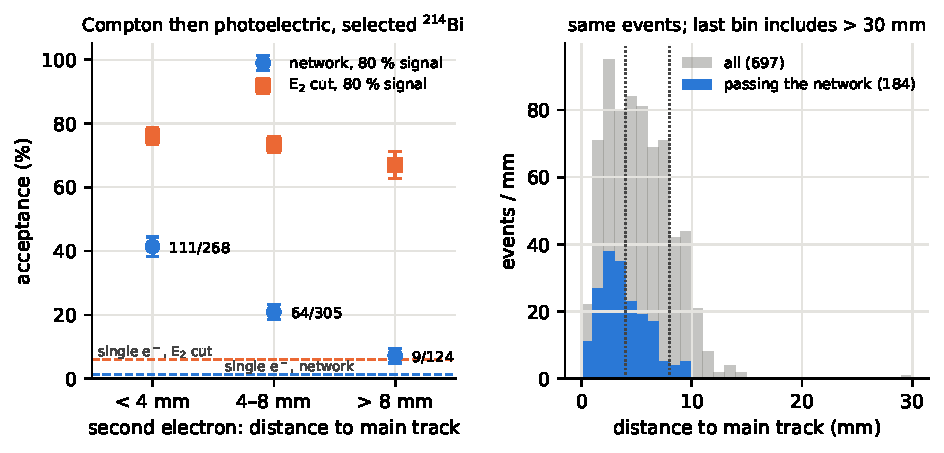
\includegraphics[width=\textwidth]{bi214_floor_distance}
\caption{Compton events of the selected \BI sample. Left: acceptance of the
network and of the \Etwo cut, both at 80\,\% signal, in the three distance
classes of Table~\ref{tab:distance}; dashed lines: single electrons. Right:
smallest distance of the second electron to the main track, all events and
those passing the network.}
\label{fig:distance}
\end{figure}

The acceptance falls with the distance of the second electron
(Table~\ref{tab:distance}, Figure~\ref{fig:distance}). Below 4~mm, about one
cell, it is \DistANet\,\%: the network separates these events from \bbonu by a
factor of only \DistARejection. They are \DistAShareSelected\,\% of the
selected sample but give \DistASharePassed\,\% of the passing events, an
acceptance of \DistAContribution\,\% of the selected \BI on their own, more
than the single-electron acceptance. The \Etwo cut accepts most of them in
every class: the second electron adds energy at the start of the main track.
One variable summarises the response of the network: weighting the
single-electron acceptance in bins of the energy within 7~mm of the start of
the leading electron with the \BI distribution of that energy predicts
\ExpectedNet$\pm$\ExpectedNetErr\,\%, against \BiNet\,\% measured.

\section{The mechanism}
\label{sec:mechanism}

\subsection{The scattered photon}
A Compton scattering of the 2447.86~keV line through an angle $\theta$ leaves
a photon of energy
\begin{equation}
E'(\theta) = \frac{E_\gamma}{1 + (E_\gamma/m_ec^2)(1-\cos\theta)},
\label{eq:compton}
\end{equation}
from energy and momentum conservation. Above $90^\circ$, $E'$ is between
\BackscatterKeV\ and \NinetyKeV~keV (Figure~\ref{fig:attenuation}, left). In xenon at
16~bar and 290~K, the attenuation length of such a photon,
$\lambda = 1/(\mu\rho)$ with $\mu/\rho$ from the NIST tables~\cite{NIST:XrayMassCoef}
and $\rho = \GasDensity$~kg/m$^3$ from the detector cards, is
\BackscatterLambda~cm at \BackscatterKeV~keV, \LambdaThree~cm at 300~keV and
\LambdaFour~cm at 400~keV (Figure~\ref{fig:attenuation}, right). The
probability of a first interaction within 1~cm is \PtenThree\,\% at 300~keV
and \PtenFour\,\% at 400~keV. The 2447.86~keV line itself has
$\lambda = \LineLambda$~cm.

\begin{figure}[htbp]
\centering
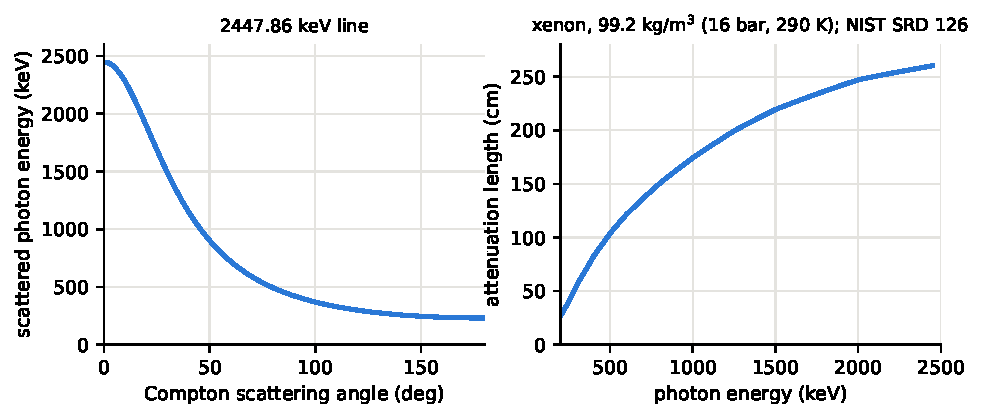
\includegraphics[width=\textwidth]{bi214_floor_attenuation}
\caption{Left: energy of the scattered photon, Eq.~\eqref{eq:compton}.
Right: attenuation length in the gas of II\_L1000\_D500, total attenuation
with coherent scattering~\cite{NIST:XrayMassCoef}, interpolated linearly in
$\log\mu/\rho$ against $\log E$.}
\label{fig:attenuation}
\end{figure}

\subsection{What the selection keeps}
Figure~\ref{fig:mechanism} shows the four outcomes of a Compton scattering
inside the gas. The scattered photon usually travels tens of centimetres. If it
escapes, the event falls below the ROI (d); if it is absorbed outside the
160~mm frame, the gamma veto rejects the event (c); if it is absorbed inside
the frame but centimetres away, the second electron forms a separate segment
and the track selection rejects the event (b). Only when the photon is
absorbed close to the vertex, typically within 1~cm (a), does the event
survive. The selection
therefore keeps a small and specific subset of the Compton events: those whose
two electrons start from almost the same point.

\begin{figure}[htbp]
\centering
% Schematic of the selection of Compton events of the 214Bi line (bi214_compton_floor.tex).
% Not to scale. Requires tikz with the libraries decorations.pathmorphing, arrows.meta, positioning.
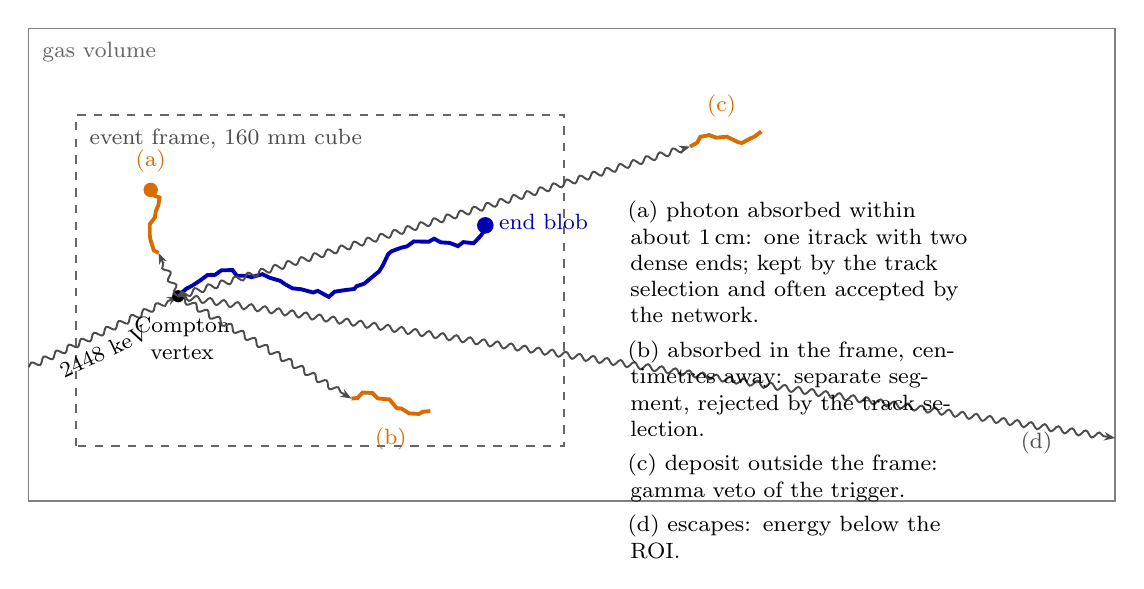
\begin{tikzpicture}[
    font=\footnotesize,
    electron/.style={draw=blue!70!black, line width=1.4pt, decorate, decoration={random steps, segment length=3pt, amplitude=1.2pt}},
    second/.style={draw=orange!85!black, line width=1.4pt, decorate, decoration={random steps, segment length=2.5pt, amplitude=1pt}},
    photon/.style={draw=black!70, line width=0.7pt, decorate, decoration={snake, amplitude=1.1pt, segment length=5pt, post length=2pt}, -{Stealth[length=4pt]}},
    note/.style={align=left, text width=4.3cm, inner sep=1pt}]
  % detector boundary and event frame
  \draw[black!50, line width=0.6pt] (-1.2,-2.6) rectangle (12.6,3.4);
  \node[anchor=north west, black!60] at (-1.15,3.35) {gas volume};
  \draw[black!60, dashed, line width=0.7pt] (-0.6,-1.9) rectangle (5.6,2.3);
  \node[anchor=north west, black!70] at (-0.55,2.25) {event frame, 160 mm cube};
  % incoming gamma
  \draw[photon] (-1.2,-0.9) -- node[below, sloped, pos=0.45] {2448 keV} (0.7,0.0);
  % Compton vertex and main electron
  \fill (0.7,0.0) circle (2.2pt);
  \node[anchor=north, align=center] at (0.75,-0.15) {Compton\\ vertex};
  \draw[electron] (0.7,0.0) .. controls (1.6,0.9) and (2.4,-0.6) .. (3.3,0.4) .. controls (3.9,1.1) and (4.4,0.3) .. (4.6,0.9);
  \fill[blue!70!black] (4.6,0.9) circle (3pt);
  \node[blue!70!black, anchor=west] at (4.65,0.95) {end blob};
  % (a) absorbed within about 1 cm
  \draw[photon] (0.7,0.0) -- (0.45,0.55);
  \draw[second] (0.45,0.55) .. controls (0.2,0.9) and (0.6,1.15) .. (0.35,1.35);
  \fill[orange!85!black] (0.35,1.35) circle (2.6pt);
  \node[anchor=south, orange!85!black] at (0.35,1.45) {(a)};
  % (b) absorbed inside the frame, centimetres away
  \draw[photon] (0.7,0.0) -- (2.9,-1.3);
  \draw[second] (2.9,-1.3) .. controls (3.3,-1.1) and (3.5,-1.6) .. (3.9,-1.45);
  \node[anchor=north, orange!85!black] at (3.4,-1.55) {(b)};
  % (c) absorbed outside the frame
  \draw[photon] (0.7,0.0) -- (7.2,1.9);
  \draw[second] (7.2,1.9) .. controls (7.5,2.2) and (7.8,1.8) .. (8.1,2.1);
  \node[anchor=south, orange!85!black] at (7.6,2.15) {(c)};
  % (d) escapes
  \draw[photon] (0.7,0.0) -- (12.6,-1.8);
  \node[anchor=north, black!70] at (11.6,-1.6) {(d)};
  % explanations
  \node[note, anchor=north west] at (6.4,1.25) {%
    (a) photon absorbed within about 1\,cm: one itrack with two dense ends; kept by the track selection and often accepted by the network.\\[3pt]
    (b) absorbed in the frame, centimetres away: separate segment, rejected by the track selection.\\[3pt]
    (c) deposit outside the frame: gamma veto of the trigger.\\[3pt]
    (d) escapes: energy below the ROI.};
\end{tikzpicture}

\caption{Outcomes of a Compton scattering of the \BI line in the gas (not to
scale). Blue: Compton electron; orange: electron from the absorption of the
scattered photon (wavy lines).}
\label{fig:mechanism}
\end{figure}

The truth confirms it. The distance from the start of the leading electron to
the energy centre of the second electron has a median of
\ComptCentreMedianAll~mm for the selected Compton events, and 90\,\% of the
passing ones are within \ComptCentreNinetyPassed~mm
(Figure~\ref{fig:centre}). This distance includes the photon path and half the
range of the second electron. Among the selected Compton events,
\ComptLtFour\,\% have the second electron within 4~mm of the main track.

\begin{figure}[htbp]
\centering
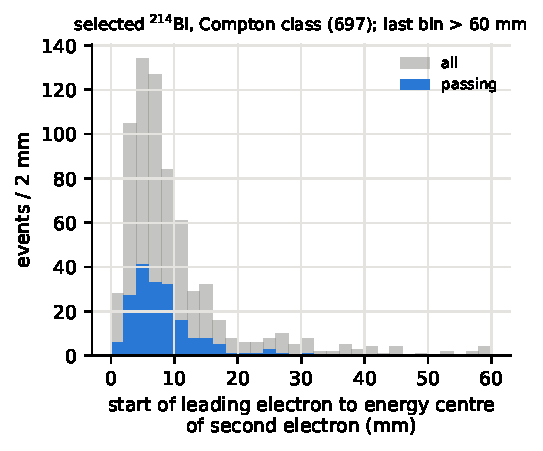
\includegraphics[width=0.5\textwidth]{bi214_floor_centre}
\caption{Selected \BI Compton events: distance from the start of the leading
electron to the energy-weighted centre of the second electron.}
\label{fig:centre}
\end{figure}

\subsection{Why it is almost irreducible}
An event of class (a) has two electrons with a common origin: one track with
a dense end at each stopping point, and extra energy at the junction. That is
the topology of \bbonu. When the second electron starts within one or two
cells of the main track, the lattice records one connected object; the
information that remains is the energy near the junction, which the network
uses (Section~\ref{sec:truth}) but which overlaps with the energy loss of the
two \bbonu electrons near their common vertex. The acceptance of
\DistANet\,\% below 4~mm, half the signal efficiency, measures what is left.
The events at 4--8~mm and beyond start at a point separated from the main
track; training against \BI, or a variable that counts track ends or measures
the separation of the two starts, could reduce them.

Figure~\ref{fig:displays} shows four events of batch 301. The two Compton
events that pass have the scattered photon absorbed \DispAPhotonPath~mm and
\DispBPhotonPath~mm from the Compton vertex, with second electrons of
\DispASecondKeV\ and \DispBSecondKeV~keV; on the lattice they are one track.
The rejected Compton event had its photon absorbed \DispRPhotonPath~mm away.

\begin{figure}[p]
\centering
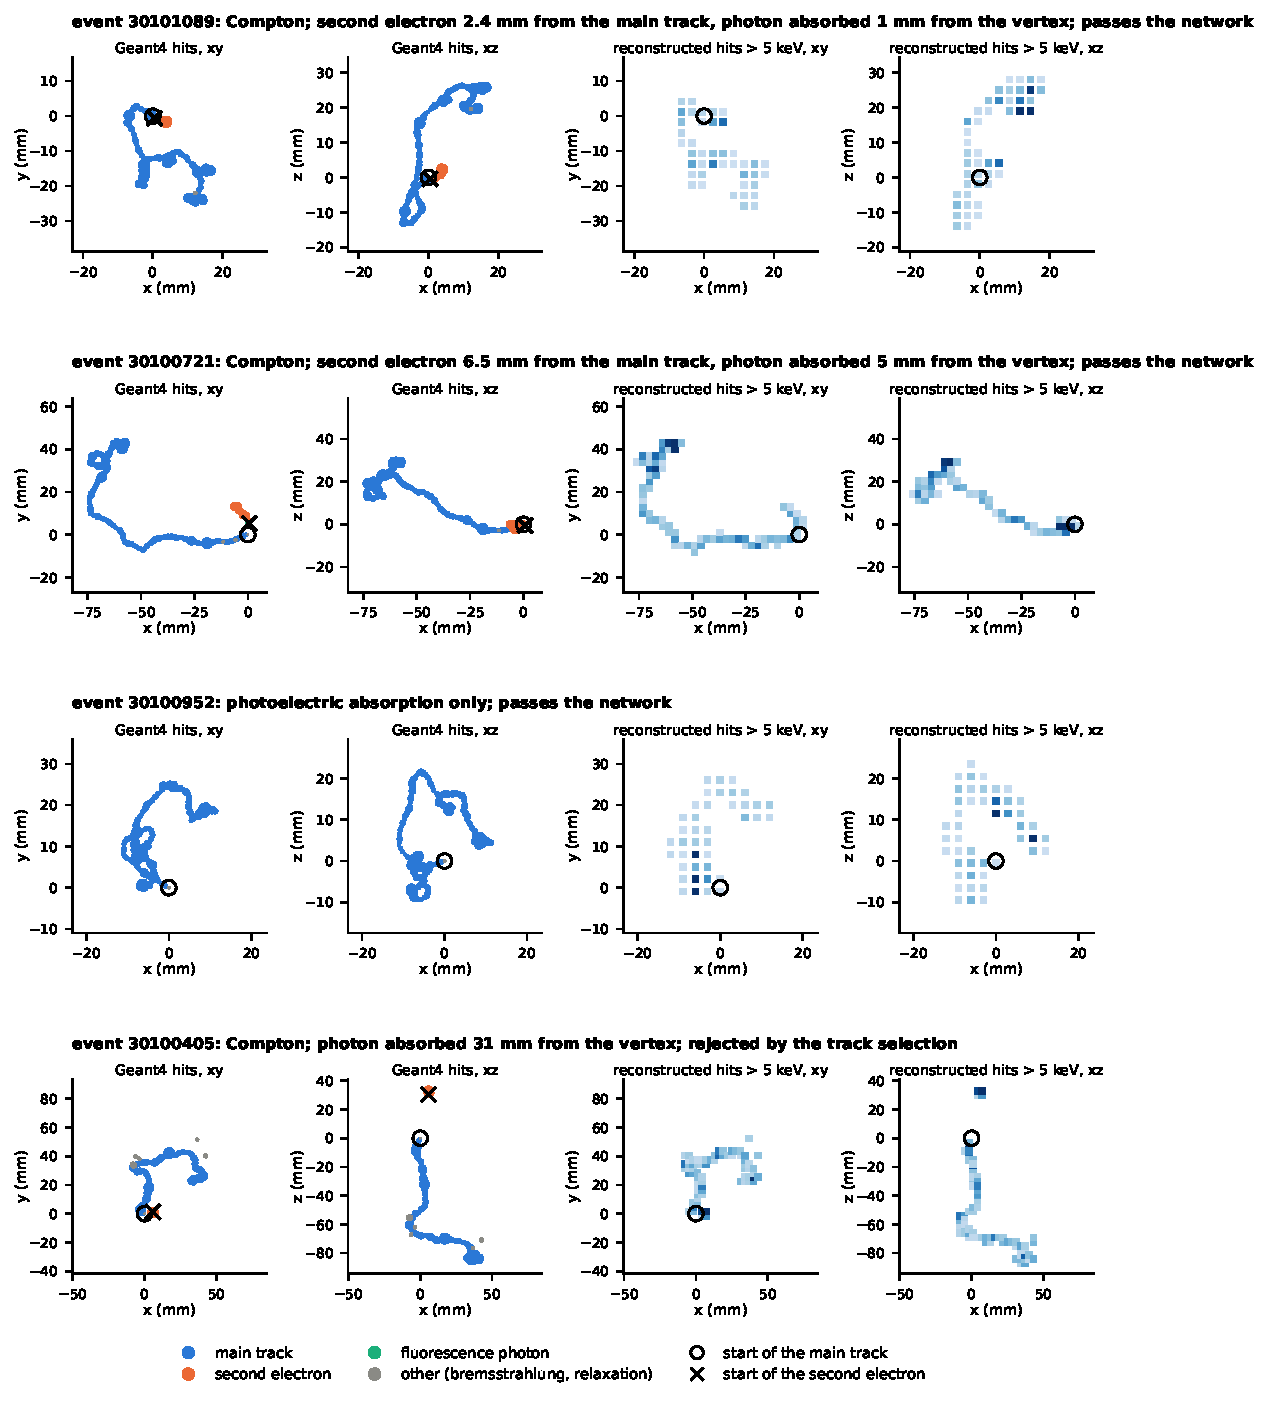
\includegraphics[width=\textwidth]{bi214_floor_displays}
\caption{Events of the \BI production (batch 301), projections $xy$ and $xz$
relative to the start of the leading electron (circle). Left two columns:
Geant4 hits, area proportional to energy, coloured by the particle that
starts them; cross: start of the second electron. Right two columns: the
reconstructed itrack hits above 5~keV of the same event on the 3~mm
lattice, shaded by energy. Rows 1--2: Compton events in the ROI that pass the
track selection and the network; row 3: a photoelectric event that passes;
row 4: a Compton event in the ROI rejected by the track selection.}
\label{fig:displays}
\end{figure}

\section{Diffusion is not the driver}
\label{sec:diffusion}
The thermal spread of the ions grows as the square root of the drift length.
If the diffusion set the background, the acceptance would change along the
drift. Table~\ref{tab:thirds} and Figure~\ref{fig:thirds} give the network
acceptance of the single electrons of the test sample in thirds of the drift
length (equal numbers of events, threshold of 80\,\% signal over all test
events), for II\_L1000\_D500 and for the ITACA detector in Xe--15\,\%~He
(16~bar, 350~V/cm, 1.3~m; runs \code{bb0nu_itaca_100k_ion15} and
\code{single_electrons_itaca_100k_ion15}, network in
\code{results/network/II_L1500_D400/}), whose ion spread reaches
\ThirdHybridFullSigma~mm at full drift.

\begin{table}[htbp]
\centering
\caption{Single electrons accepted by the network at 80\,\% signal in thirds
of the drift length; $\sigma$: thermal ion spread at the median drift of the
third; last column: signal efficiency in the third.}
\label{tab:thirds}
\begin{tabular}{llrrrr}
\toprule
Detector & Drift (cm) & $\sigma$ (mm) & Events & Accepted (\%) & Signal (\%) \\
\midrule
II\_L1000\_D500 & \ThirdPureOneLo--\ThirdPureOneHi & \ThirdPureOneSigma & \ThirdPureOneEvents & \ThirdPureOne$\pm$\ThirdPureOneErr & \ThirdPureOneSig \\
pure xenon & \ThirdPureTwoLo--\ThirdPureTwoHi & \ThirdPureTwoSigma & \ThirdPureTwoEvents & \ThirdPureTwo$\pm$\ThirdPureTwoErr & \ThirdPureTwoSig \\
 & \ThirdPureThreeLo--\ThirdPureThreeHi & \ThirdPureThreeSigma & \ThirdPureThreeEvents & \ThirdPureThree$\pm$\ThirdPureThreeErr & \ThirdPureThreeSig \\
 & all & & & \ThirdPureAll$\pm$\ThirdPureAllErr & 80.0 \\
\midrule
ITACA & \ThirdHybridOneLo--\ThirdHybridOneHi & \ThirdHybridOneSigma & \ThirdHybridOneEvents & \ThirdHybridOne$\pm$\ThirdHybridOneErr & \ThirdHybridOneSig \\
Xe--15\,\%~He & \ThirdHybridTwoLo--\ThirdHybridTwoHi & \ThirdHybridTwoSigma & \ThirdHybridTwoEvents & \ThirdHybridTwo$\pm$\ThirdHybridTwoErr & \ThirdHybridTwoSig \\
 & \ThirdHybridThreeLo--\ThirdHybridThreeHi & \ThirdHybridThreeSigma & \ThirdHybridThreeEvents & \ThirdHybridThree$\pm$\ThirdHybridThreeErr & \ThirdHybridThreeSig \\
 & all & & & \ThirdHybridAll$\pm$\ThirdHybridAllErr & 80.0 \\
\bottomrule
\end{tabular}
\end{table}

\begin{figure}[htbp]
\centering
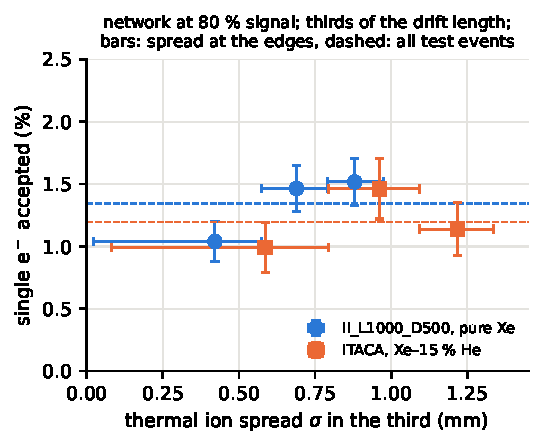
\includegraphics[width=0.55\textwidth]{bi214_floor_thirds}
\caption{Data of Table~\ref{tab:thirds} against the thermal ion spread.}
\label{fig:thirds}
\end{figure}

There is no consistent trend with the spread between 0.4 and 1.2~mm. In
II\_L1000\_D500 the acceptance rises from the first to the last third by
1.9 standard deviations; in ITACA the third with the largest spread
(\ThirdHybridThreeSigma~mm) is below the middle one, and the overall
acceptance, \ThirdHybridAll\,\% at \ThirdHybridFullSigma~mm full-drift spread,
is that of II\_L1000\_D500 (\ThirdPureAll\,\% at \ThirdPureFullSigma~mm).
The \BI events show the same behaviour. In thirds of the drift of the
\BiThirdRoi\ ROI events each, the network accepts
\BiThirdOneNet$\pm$\BiThirdOneNetErr, \BiThirdTwoNet$\pm$\BiThirdTwoNetErr\ and
\BiThirdThreeNet$\pm$\BiThirdThreeNetErr\,\% of the selected events, and
\BiThirdOnePerRoi, \BiThirdTwoPerRoi\ and \BiThirdThreePerRoi\ per thousand ROI
events pass both the track selection and the network. The diffusion acts on
the track selection, which keeps \BiThirdOneSel, \BiThirdTwoSel\ and
\BiThirdThreeSel\,\% of the ROI events from the shortest to the longest drift;
the Compton class grows faster (\BiThirdOneComptShare,
\BiThirdTwoComptShare\ and \BiThirdThreeComptShare\,\% of the selected), and
the network accepts it less often at long drift
(\BiThirdOneComptNet$\pm$\BiThirdOneComptNetErr,
\BiThirdTwoComptNet$\pm$\BiThirdTwoComptNetErr\ and
\BiThirdThreeComptNet$\pm$\BiThirdThreeComptNetErr\,\%), so that the product
does not change.

The spread is at most a third of the 3~mm pitch, $\sigma/p \le 0.33$. The
smallest separation the readout resolves is one empty cell between two
deposits, set by the pitch; the diffusion moves charge across a cell boundary
but does not change that scale.

\section{The voxelised Monte Carlo}
\label{sec:voxel}
To see what a voxelised response would conclude, the Geant4 hits of the
\VoxEvents\ \BI events in the ROI were summed in 3~mm cells of a lattice fixed
in detector coordinates, inside the simulated box of each event; cells above
3~keV are the hits, and the track selection of the production is applied to
them with the same settings (\code{scripts/iitaca/prepare_bi214_floor.jl}).
The energy of the cells equals the energy in the box of the production for
every event (largest difference \VoxBoxDiff~keV). The comparison is of the
track selection only; the network was not applied to the voxelised events.

\begin{table}[htbp]
\centering
\caption{Track selection of the \VoxEvents\ \BI events in the ROI: full readout
against the voxelised Monte Carlo.}
\label{tab:voxel}
\begin{tabular}{lrr}
\toprule
 & Full readout & Voxelised Monte Carlo \\
\midrule
Selected & \VoxReadoutSelected & \VoxSelected \\
Selected by both & \multicolumn{2}{c}{\VoxBoth} \\
Selected by one only & \ReadoutOnly & \VoxOnly \\
Selected, drift thirds (\%) & \BiThirdOneSel, \BiThirdTwoSel, \BiThirdThreeSel & \BiThirdOneVox, \BiThirdTwoVox, \BiThirdThreeVox \\
\midrule
\multicolumn{3}{l}{Events selected by the full readout, kept by the voxelised selection:} \\
\quad Compton class & \ComptEvents & \VoxComptKept\ (\VoxComptKeptFrac\,\%) \\
\quad\quad second electron $<4$~mm & \VoxDistAEvents & \VoxDistAKept\,\% \\
\quad\quad 4--8~mm & \VoxDistBEvents & \VoxDistBKept\,\% \\
\quad\quad $>8$~mm & \VoxDistCEvents & \VoxDistCKept\,\% \\
\quad other classes & & \VoxPhotKept\,\% \\
\quad passing the network & \BiNetPassed & \VoxPassKept \\
\quad\quad of which Compton & \ComptPassed & \VoxComptPassKept \\
\bottomrule
\end{tabular}
\end{table}

Table~\ref{tab:voxel} gives the result. The voxelised Monte Carlo selects
\VoxSelected\ events against \VoxReadoutSelected. Of the \ReadoutOnly\ events
that only the full readout selects, \VoxRejDeposit\ are rejected in the
voxelised Monte Carlo by a detached deposit. In the full readout, a deposit
of a few tens of keV near the track is spread by the diffusion over several
cells, some below the 5~keV cut, and its charge reaches cells that touch the
track; the ion statistics, the noise and the lattice phase move it further. The
selected fraction of the full readout rises with the drift, that of the
voxelised Monte Carlo does not, which identifies the diffusion as the
cause of the growth: the events selected only by the full readout are
\BiThirdOneReadoutOnly, \BiThirdTwoReadoutOnly\ and \BiThirdThreeReadoutOnly\,\%
of the ROI events in the three thirds of the drift. In the first third, where the
spread is below 0.55~mm, the difference is already \BiThirdOneReadoutOnly\,\%;
it also contains the other differences between the two responses: ion
statistics, noise and lattice phase.

The difference is concentrated where it matters. The voxelised selection keeps
\VoxComptKeptFrac\,\% of the Compton events that the full readout keeps, and
only \VoxDistCKept\,\% of those with the second electron beyond 8~mm. Of the
\ComptPassed\ Compton events that pass the network in the full simulation,
\VoxComptPassKept\ survive the voxelised track selection. A study based on the
voxelised response would start the separation stage with one third fewer
events of the class that dominates the surviving background, and with a
different mixture of its distance classes; it has no handle on the response
of a network to the events that the full readout keeps and it removes. The
background measured that way is an underestimate whose size can only be
obtained from the full chain.

\section{The readout pitch}
\label{sec:pitch}
The irreducible part is the Compton events whose second electron starts
within one or two cells of the main track; the distance classes of
Table~\ref{tab:distance} are in units of the 3~mm pitch. A run with 2~mm pads,
II\_L1000\_D500\_P2, tests it.

\paragraph{Prediction.} If the network acceptance of a Compton event depends
on the distance of its second electron in units of the pitch, the classes
of Table~\ref{tab:distance} move to $<\PitchEdgeOne$~mm,
\PitchEdgeOne--\PitchEdgeTwo~mm and $>\PitchEdgeTwo$~mm at 2~mm. With the
selected events of the 3~mm production, these hold \PitchDistAEvents,
\PitchDistBEvents\ and \PitchDistCEvents\ Compton events, and the measured
acceptances give \PitchComptPassed\ passing Compton events instead of
\ComptPassed. With the \PitchOthers\ passing events of the other classes
unchanged, the \BI acceptance would fall from \BiNet\ to about \PitchTotalNet\,\%.
About \PitchIrreducible\ events, those below \PitchEdgeOne~mm, would remain.
The estimate keeps the 3~mm selected sample; a finer lattice also rejects more
Compton events at the track selection, and the ion spread at full drift
becomes half the 2~mm pitch.

\paragraph{Comparison with II\_L1000\_D500\_P2.}
The 2~mm run reads the same Geant4 events, with the same seeds and ion drift,
on 2~mm pads with 10~ms frames (2~mm along the drift). Hits are kept above
3~keV, and the track selection uses a hit cut of 3~keV, since at 5~keV the
smaller cells break the track. Its radii are scaled to the lattice: components
at 3.7~mm, segments of at least 9 hits, joined at \TwoSegJoin~mm; the
detached-deposit threshold (10~keV) and the end-point spheres (7~mm) are
unchanged. A network of the same architecture is trained on the 2~mm itracks
of \bbonu and single electrons, and the truth study is repeated on the
selected \BI events (\code{results/iitaca/II_L1000_D500_pitch_comparison/}).
Table~\ref{tab:pitch} compares the two pitches.

\begin{table}[htbp]
\centering
\caption{\BI and single electrons on 3~mm and 2~mm pads, same Geant4 events and
\BiROI\ \BI events in the ROI. Acceptances at 80\,\% signal; the network
acceptance of single electrons is that of the test sample of each training.}
\label{tab:pitch}
\begin{tabular}{lrr}
\toprule
 & 3~mm & 2~mm \\
\midrule
\bbonu: track selection (\% of the ROI) & \BbSelFrac & \TwoBbSelFrac \\
\BI: track selection (events, \% of the ROI) & \BiSelected\ (\BiTrackFraction) & \TwoBiSelected\ (\TwoBiTrackFraction) \\
\Etwo threshold (keV) & \EtwoThreshold & \TwoEtwoThreshold \\
\Etwo cut: \BI, single electrons (\%) & \BiEtwo, \SeEtwo & \TwoBiEtwo, \TwoSeEtwo \\
Network: single electrons (\%) & \SeNet$\pm$\SeNetErr & \TwoSeNet$\pm$\TwoSeNetErr \\
Network: \BI (\%) & \BiNet$\pm$\BiNetErr\ (\BiNetPassed) & \TwoBiNet$\pm$\TwoBiNetErr\ (\TwoBiNetPassed) \\
\quad photoelectric absorption only & \PhotNet\ (\PhotPassed/\PhotEvents) & \TwoPhotNet\ (\TwoPhotPassed/\TwoPhotEvents) \\
\quad Compton, then absorption & \ComptNet\ (\ComptPassed/\ComptEvents) & \TwoComptNet\ (\TwoComptPassed/\TwoComptEvents) \\
\quad\quad second electron $<4$~mm & \DistANet\ (\DistAPassed/\DistAEvents) & \TwoDistANet\ (\TwoDistAPassed/\TwoDistAEvents) \\
\quad\quad 4--8~mm & \DistBNet\ (\DistBPassed/\DistBEvents) & \TwoDistBNet\ (\TwoDistBPassed/\TwoDistBEvents) \\
\quad\quad $>8$~mm & \DistCNet\ (\DistCPassed/\DistCEvents) & \TwoDistCNet\ (\TwoDistCPassed/\TwoDistCEvents) \\
\BI passing the network, per 1000 ROI events & \BiPerRoi & \TwoBiPerRoi \\
\bottomrule
\end{tabular}
\end{table}

The track selection keeps fewer \BI events at 2~mm, \TwoBiSelected\ against
\BiSelected, and the loss is in the Compton class: \TwoComptEvents\ events
against \ComptEvents. Segments joined at \TwoSegJoin~mm instead of 8~mm leave
apart the second electrons that start away from the main track: the class
beyond 8~mm falls from \DistCEvents\ to \TwoDistCEvents\ events and the 4--8~mm
class from \DistBEvents\ to \TwoDistBEvents, while the class below 4~mm falls
only from \DistAEvents\ to \TwoDistAEvents. The Compton events that remain are
the harder ones and pass the network at \TwoComptNet\,\%, against \ComptNet\,\%.
Below 4~mm the acceptance is \TwoDistANet$\pm$\TwoDistANetErr\,\%, against
\DistANet$\pm$\DistANetErr\,\% at 3~mm: when the second electron touches the
main track, the finer lattice does not separate it. These \TwoDistAPassed\ of
the \TwoBiNetPassed\ passing events are the floor. Photoelectric events
pass at \TwoPhotNet\,\%, against \TwoSeNet\,\% for single electrons
(\PhotNet\ and \SeNet\,\% at 3~mm).

In units of the pitch (Figure~\ref{fig:pitch}, right) the acceptance below
$4/3$ of the pitch is the same at both pitches, \TwoPitchANet$\pm$\TwoPitchANetErr\,\%
at 2~mm (\TwoPitchAPassed\ of \TwoPitchAEvents, below \PitchEdgeOne~mm), as the
prediction assumed. Beyond, the 2~mm acceptance is higher,
\TwoPitchBNet\ and \TwoPitchCNet\,\% against \DistBNet\ and \DistCNet\,\%,
because the track selection has already removed most of the separated events.
The prediction gave \PitchComptPassed\ passing Compton events and
\PitchIrreducible\ below \PitchEdgeOne~mm; the run gives \TwoComptPassed\ and
\TwoPitchAPassed. Per thousand ROI events, \TwoBiPerRoi\ \BI events pass the
track selection and the network at 2~mm, against \BiPerRoi\ at 3~mm and
\PitchPerRoi\ predicted. The reduction, a factor \TwoGain, comes in equal parts
from the track selection (\TwoSelGain) and from the network (\TwoNetGain).

\begin{figure}[htbp]
\centering
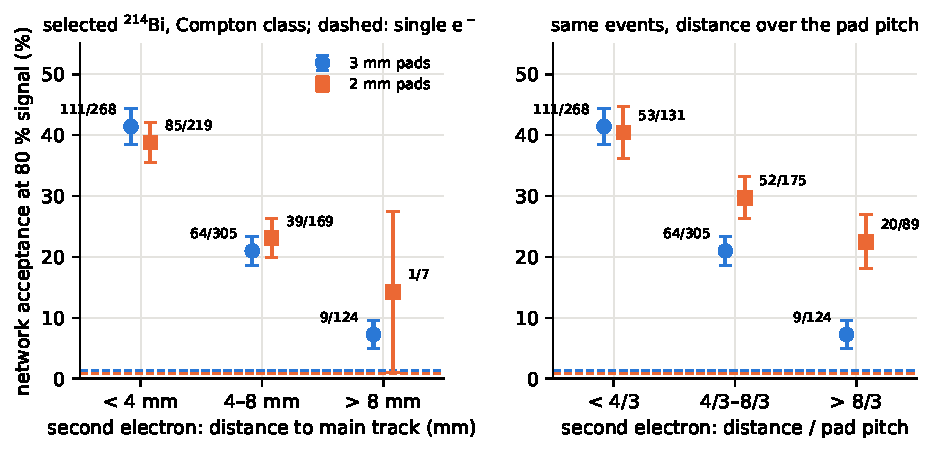
\includegraphics[width=\textwidth]{bi214_floor_pitch}
\caption{Network acceptance at 80\,\% signal of the selected \BI Compton
events on 3~mm and 2~mm pads, against the smallest distance of the second
electron to the main track. Left: in mm, the classes of
Table~\ref{tab:distance}; right: in units of the pad pitch. Labels: passing
over selected events; dashed lines: single electrons.}
\label{fig:pitch}
\end{figure}

\section{Summary}
\label{sec:summary}
\begin{enumerate}
\item After the track selection, \BI passes the network at \BiNet\,\%,
  \BiNetRatio\ times the single-electron acceptance. Compton events, \ComptShareSelected\,\%
  of the selected sample, give \ComptSharePassed\,\% of the passing events.
\item The selection keeps only the Compton events whose scattered photon,
  with an attenuation length of \BackscatterLambda\ to \LambdaFive~cm, was absorbed within about 1~cm.
  Their two electrons from almost one point mimic \bbonu; with the second
  electron within 4~mm they pass at \DistANet\,\%.
\item The acceptance does not change with the ion spread from 0.4 to 1.2~mm,
  in pure xenon and in Xe--He. The relevant scale is the pitch.
\item A voxelised Monte Carlo keeps one third fewer of these Compton events at
  the track selection; the background it gives is an underestimate.
\item With 2~mm pads, the scaling estimate gives \PitchTotalNet\,\%, with about
  \PitchIrreducible\ events from second electrons within \PitchEdgeOne~mm.
  The 2~mm run gives \TwoBiNet\,\% of a smaller selected sample,
  \TwoBiPerRoi\ instead of \BiPerRoi\ passing events per thousand in the ROI;
  second electrons below 4~mm still pass at \TwoDistANet\,\%.
\end{enumerate}

\appendix
\section{Reproduction}
\label{app:repro}
\begin{enumerate}
\item Inputs copied from Hyperion (read only) by
  \code{work/bi214_note/extract_remote.py}: the Geant4 hits of the
  \BiROI\ ROI events from \code{bi214_bNNNNN_hitdf.h5}, the NEXUS particles
  of the ROI events of batch 301, and the hit file of batch 301.
\item Reduction (Julia): \code{julia --project=. scripts/iitaca/prepare_bi214_floor.jl
  work/bi214_note/unpacked/out results/iitaca/II_L1000_D500_bi214_floor/floor.h5}.
  It reads the statistics, comparison, network scores, trainings and truth
  files of the production, records their SHA-256, and writes the cut flow, the
  acceptances, the drift thirds, the attenuation lengths, the voxelised
  selection and the event displays.
\item Presentation (Python): \code{python notes/physics/figures/build_bi214_floor.py}
  writes the figures \code{notes/physics/figures/bi214_floor_*.pdf} and the
  macros \code{notes/physics/generated/bi214_floor_values.tex}.
\end{enumerate}
The truth study is \code{scripts/iitaca/prepare_iitaca_truth.jl} and
\code{summarize_iitaca_truth.jl}; the network scores are
\code{results/network/II_L1000_D500/trainings/itrack_sparse_e100/scores_bi214.h5}.

\bibliographystyle{unsrtnat}
\bibliography{references}
\end{document}
